%/*****************************************************************************
% * WindNinja Tutorial 2
%/*****************************************************************************

\documentclass[12pt]{article}
\usepackage{float}
\usepackage{graphicx}
\usepackage[margin=1in]{geometry}

\graphicspath{{imgs/}}

\usepackage[utf8]{inputenc}
\usepackage[english]{babel}
\usepackage[parfill]{parskip}
\usepackage{datetime}
\usepackage{hyperref}
\hypersetup{
	colorlinks=true,
	urlcolor=blue,
  }
\urlstyle{same}
\usepackage{subcaption} 
\usepackage{dirtytalk}
\usepackage{multirow}
\usepackage{booktabs}


\usepackage{fancyhdr}
\pagestyle{fancy}
\fancyhf{}
\rhead{WindNinja Tutorial 2: Diurnal Winds and Non-neutral Stability}
\cfoot{\thepage}

\newcommand\vn{3.6.0}

\begin{document}
\begin{titlepage}
    \centering
    {\Huge
       WindNinja Tutorial 2: Diurnal Winds and Non-neutral Stability
    }    
    \vfill
    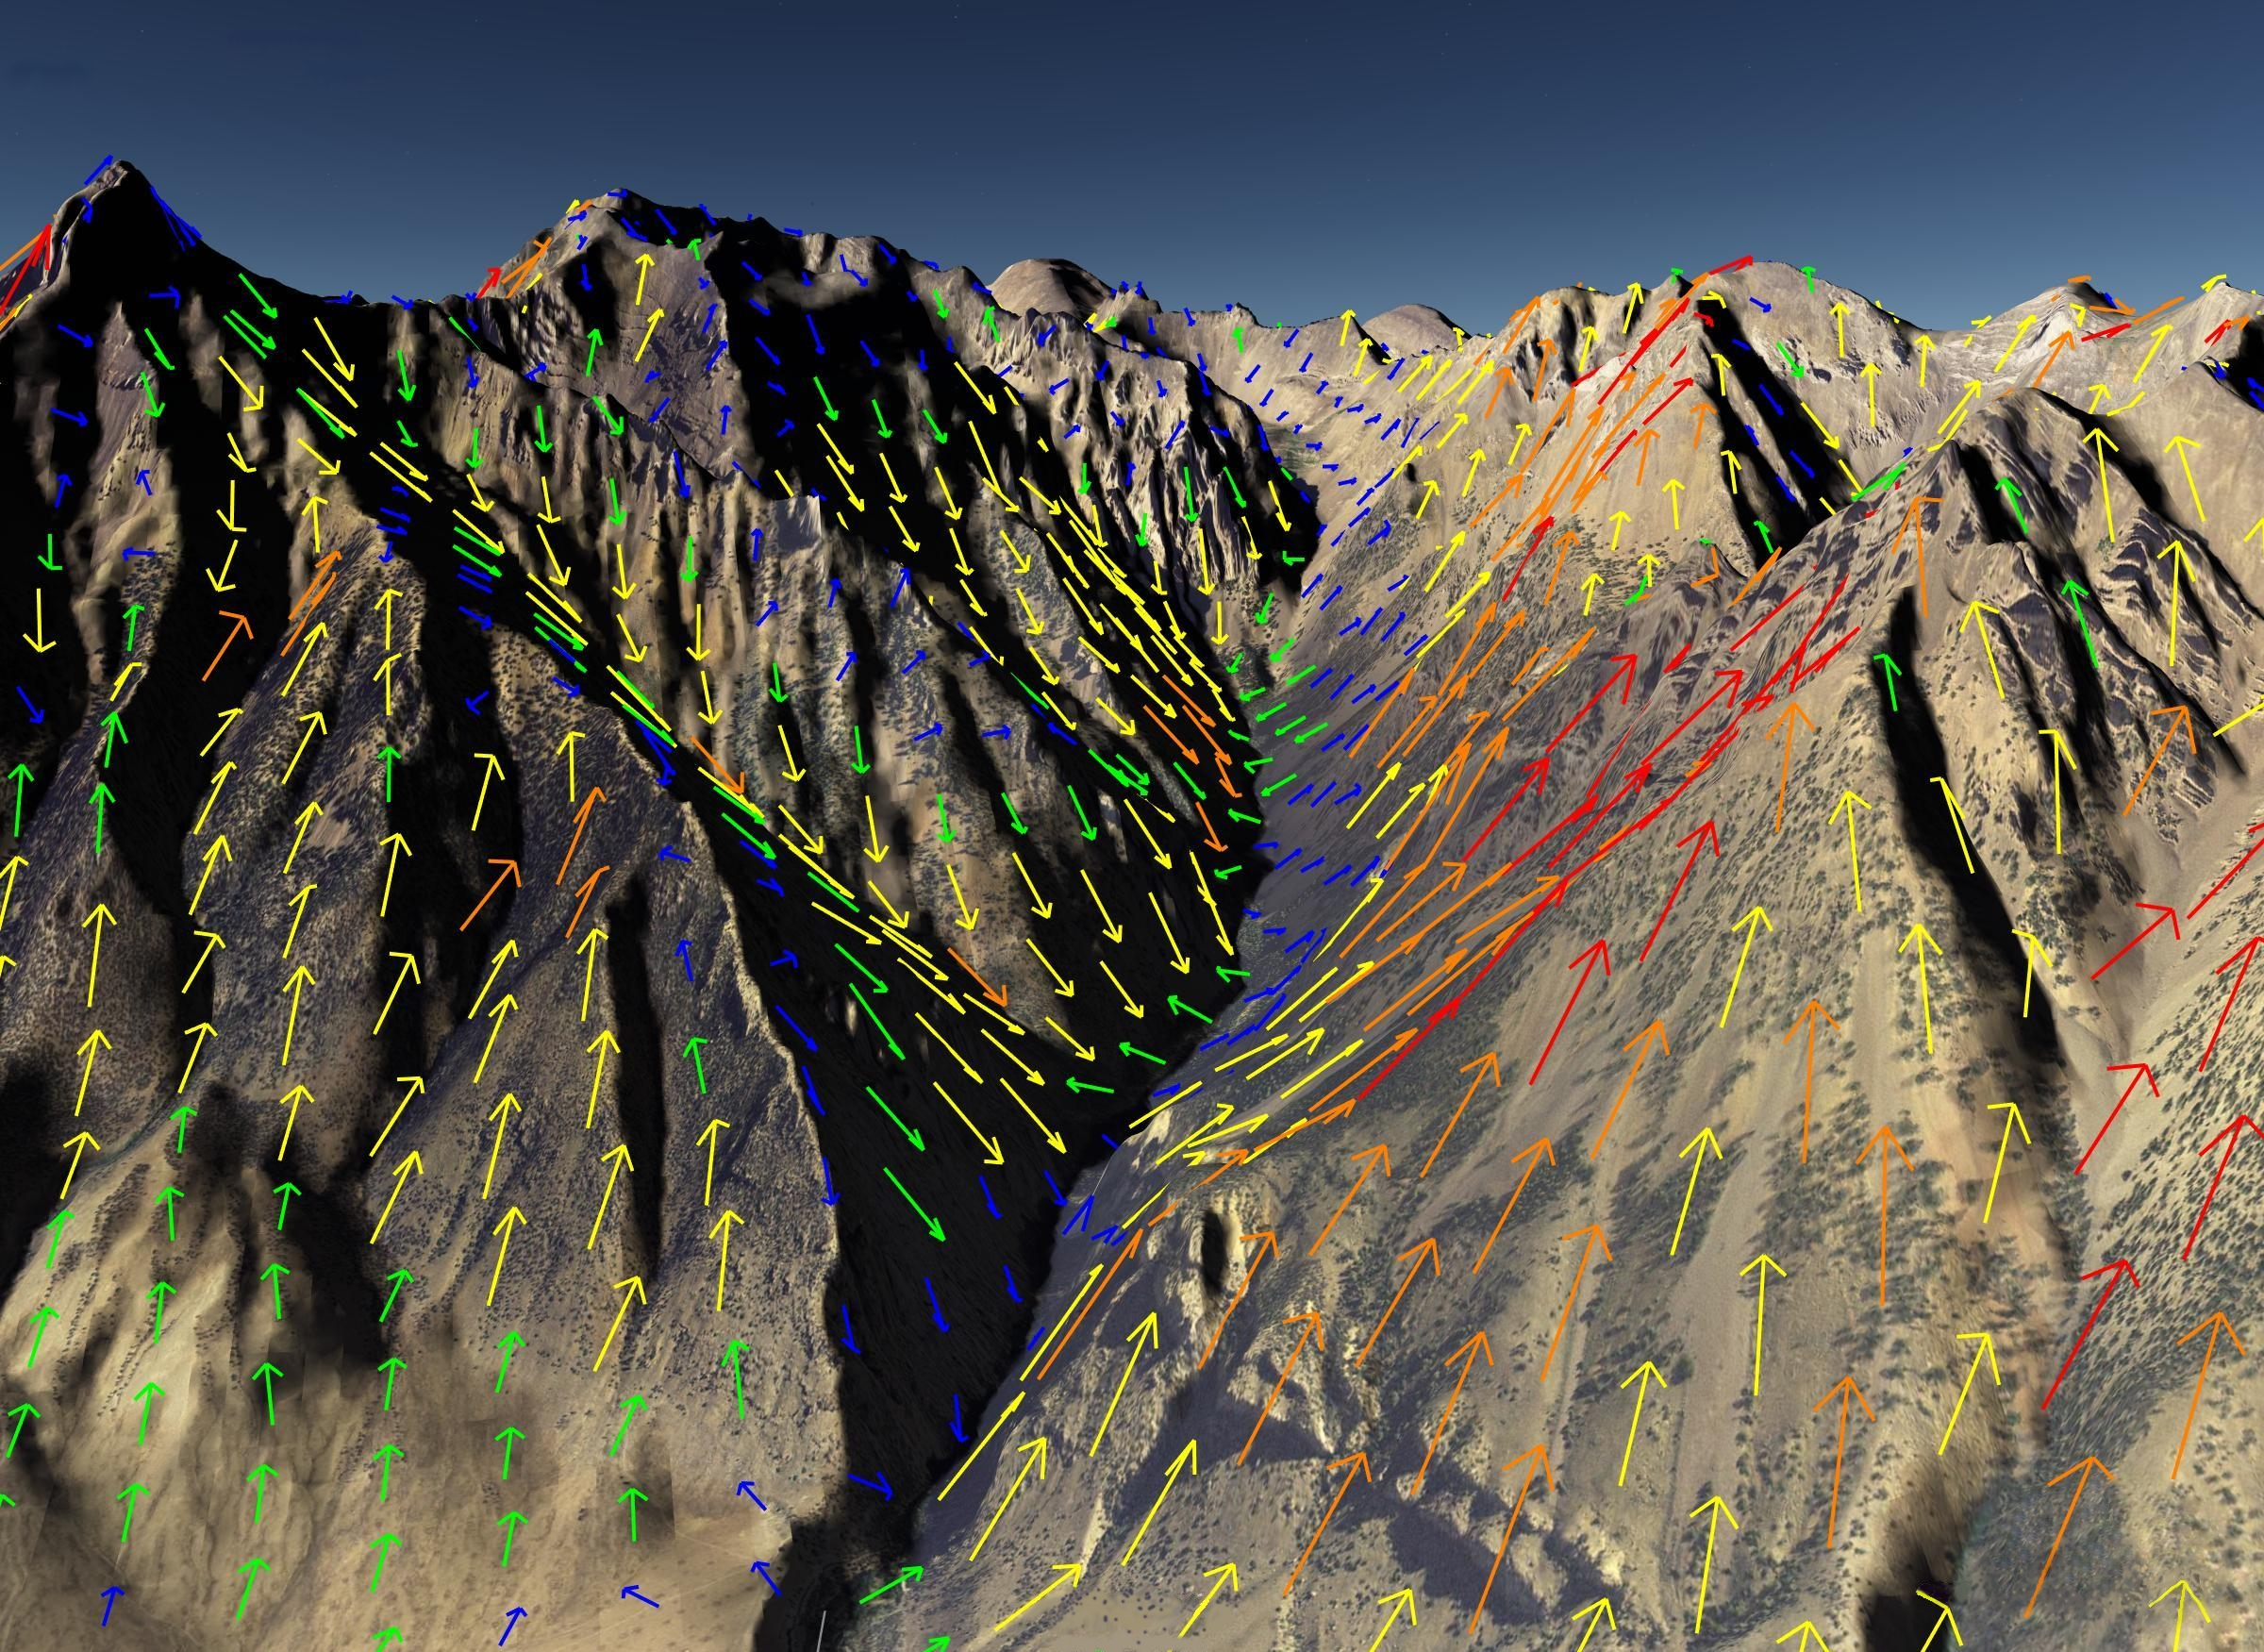
\includegraphics[scale=0.2]								{imgs/title_fig.jpg}
    \vfill
  	{\Huge
	  3/25/2020 %Date Last Edited
  	}
    \vfill
\end{titlepage}

\section*{Introduction}
Welcome to WindNinja Tutorial 2: Diurnal Winds and Non-neutral Stablity.  This tutorial will step you through the process of running a WindNinja simulation that includes diurnal slope winds and an atmospheric stability that is not neutral.  For the purposes of this tutorial, a domain average wind initialization run will be shown, but diurnal wind and non-neutral stability can be included with the other WindNinja initialization methods discussed in subsequent tutorials (point initialization, weather model initialization).  Note that the non-neutral stability option is not currently available for use with the momentum solver. This tutorial assumes you have already gone through \href{https://weather.firelab.org/windninja/tutorials/WindNinja_tutorial1.pdf}{WindNinja Tutorial 1: The Basics}.  After this tutorial, you should feel comfortable incorporating the diurnal wind and non-neutral stability submodels in your WindNinja runs.

Note:  All required user actions in this tutorial are shown in  \textbf{\color{red} red}.

\section*{What are Diurnal Winds?}

Most firefighters already have a good understanding of what diurnal slope winds are, because they are discussed in fire behavior training courses and experienced often on fires.  Diurnal slope winds are caused by warming of mountain slopes by daytime sunlight or cooling by nocturnal radiation (that is, radiation emitted by the \say{warm} ground that is lost to the \say{cold} sky).  This heats or cools the air adjacent to the slope, causing buoyant forces that produce flow up or down the slope.  During the daytime, a slope’s orientation to the sun can affect its rate of heating and, therefore, the strength of the diurnal wind.  Other factors affecting the diurnal wind strength are how well solar energy is absorbed by the ground surface and transferred to the air, how cloudy it is, and how steep the slope is.

A simple model has been included in WindNinja to simulate the effects of diurnal slope winds.  It is designed to compute small scale slope winds, but not larger scale valley winds.  The slope winds will have some effect of producing valley winds, but it will be slight.  Also, the model will not simulate other buoyancy driven flows such as sea or land breezes.

Use of the diurnal wind model in WindNinja adds additional input requirements.  Most of these inputs (date, time, latitude/longitude, etc.) are the result of having to compute the solar angle at locations across the terrain.

\section*{What Does the Non-neutral Stability Model Do?}

Atmospheric stability is a measure of the resistance of the atmosphere to vertical motion.  This is caused by varying air density with height above the ground.  Atmospheric stability can have a dramatic impact on surface wind flow.  In a very stable atmosphere, flow approaching a mountain would likely tend to flow around the sides rather than over the mountain.  In an unstable atmosphere, the flow might tend to go over the mountain.  This is a simplified description of what can be a fairly complex phenomena.  Some examples of the complexities of reality are:  1) in certain stable flow conditions wave and breaking-wave structures can form near terrain, 2) the atmospheric stability can change with height in the atmosphere, 3) some conditions can generate severe downslope wind conditions.

WindNinja has a simple model to include some of the simple aspects of non-neutral stability flows.  It can be easily turned on and requires few additional inputs from the user.  The current model calculates the surface heat flux to approximate the atmospheric stability.  Future models will likely use additional information to get a better picture of the state of the atmosphere (mesoscale weather models, etc.).  For this reason, the non-neutral stability model is considered in a beta test phase at this point.  The current model will approximately simulate non-neutral flows, but not the complex situations mentioned above.

\section{Getting Started}

\textbf{\color{red}Start WindNinja by going to Start $\Rightarrow$ Programs $\Rightarrow$ WindNinja \vn\ $\Rightarrow$ WindNinja \vn\ }

\section{Input}
\subsection{Surface Input}

\textbf{\color{red} In the navigation tree, left-click on \say{Surface Input}.}


\textbf{\color{red} In the input panel below, left-click on the \say{Open Elevation File} button.  In the window that opens, navigate to and select your elevation file.  Optionally, you could left-click on the \say{Download File} button to download a file from a USGS server as described in \href{https://weather.firelab.org/windninja/tutorials/fetch_dem_instructions.pdf}{download\_elevation\_file.pdf}.}

\textbf{\color{red} Select the dominant vegetation type using the \say{Vegetation} drop down list.  If your elevation file was a FARSITE landscape file, this drop-down box will be grayed out, since the vegetation information is obtained from the landscape file.  In this case, you do not need to select a vegetation type.}

\textbf{\color{red}
Select your desired mesh resolution using the \say{Mesh Resolution} drop-down list.}

For diurnal calculations, WindNinja needs time information to compute the sun angle.  Near the bottom of the surface input panel is an area to enter time zone information.  You will enter the \textit{actual time of day} for the simulation later.  By default, only time zones in the United States are shown.  To see all the available time zones in the world, you can check the \say{Show All Zones} check box.  To view information about a selected time zone, check the \say{Display time zone detail} check box.  Beginning with WindNinja 2.1, the determination of daylight savings or standard time is automatically handled based on the selected time zone and the date and time of the simulation.

\textbf{\color{red} Select the timezone that the elevation file is located in.}

If your elevation file spans two time zones, you could choose either one.  All output times will then be relative to the chosen time zone.

\subsection{Diurnal Input}

\textbf{\color{red}Left-click on \say{Diurnal Input} in the navigation tree, then check the \say{Use Diurnal Wind} check box in the input panel to activate the diurnal flow calculations.}

\begin{figure}[H]
	\centering
	\label{}
	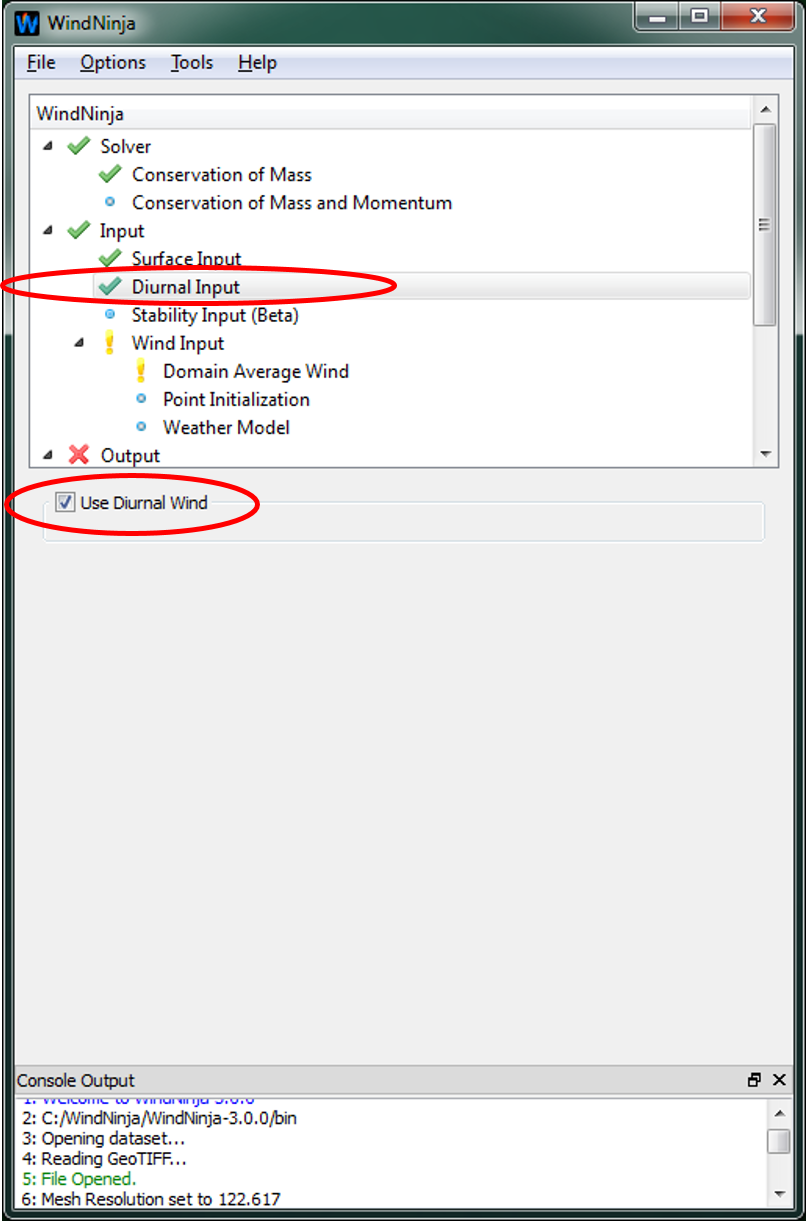
\includegraphics[scale=1.0]{imgs/diurnal_layout_1.png}
\end{figure}

\subsection{Stability Input}

\textbf{\color{red} Left-click on \say{Stability Input} in the navigation tree, then check the \say{Use Stability} check box in the input panel to activate the calculation of atmospheric stability.}

\begin{figure}[H]
	\centering
	\label{}
	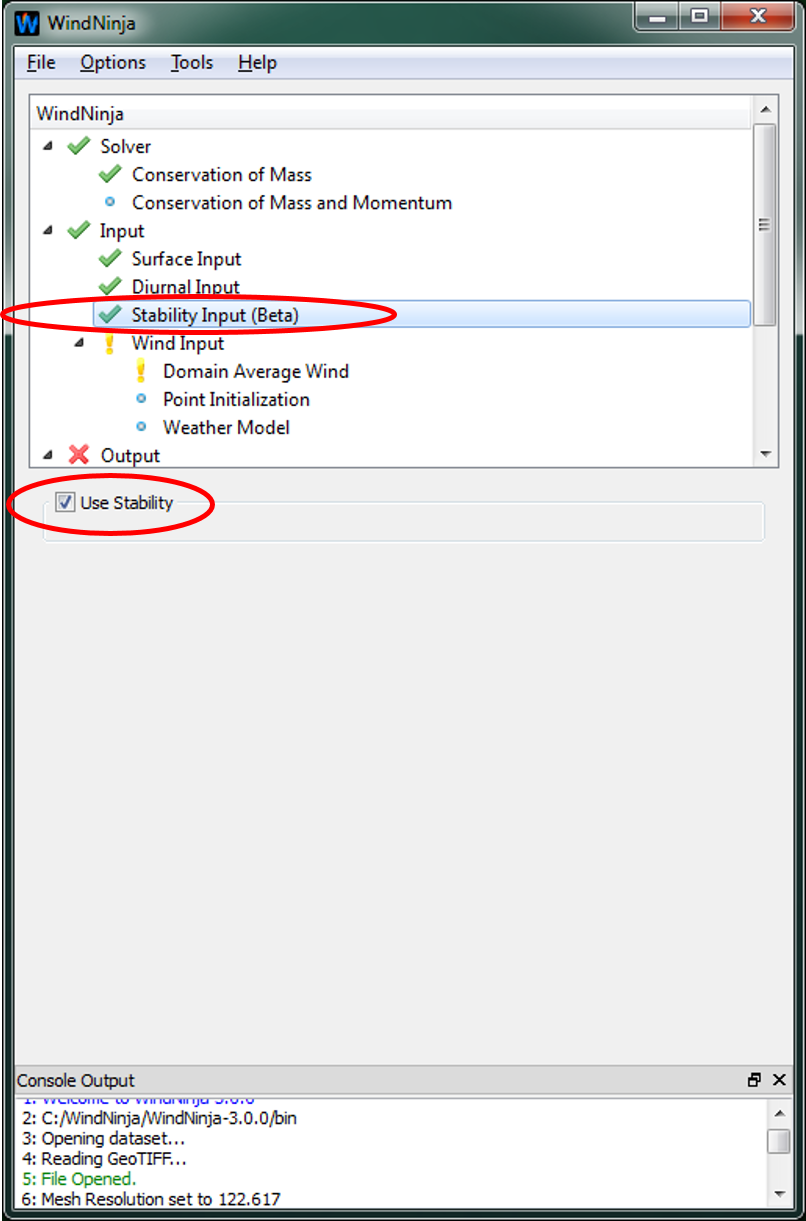
\includegraphics[scale=1.0]{imgs/stability_layout_1.png}
\end{figure}

\subsection{Wind Input}

\textbf{\color{red} Under \say{Wind Input} in the navigation tree, left-click on \say{Domain Average Wind}.  In the input panel below, check the \say{Domain Average Wind} check box to activate domain average wind initialization.}


\textbf{\color{red} In the input panel, select your input wind height using the \say{Input Wind Height} drop down list.}

\subsubsection{2.4.1. Entering Speed, Direction, and Additional Diurnal Inputs}

Because \say{Use Diurnal Wind} and \say{Use Stability} were checked earlier, additional input fields near speed and direction that are normally grayed out are now editable as shown below.

\begin{figure}[H]
	\centering
	\label{}
	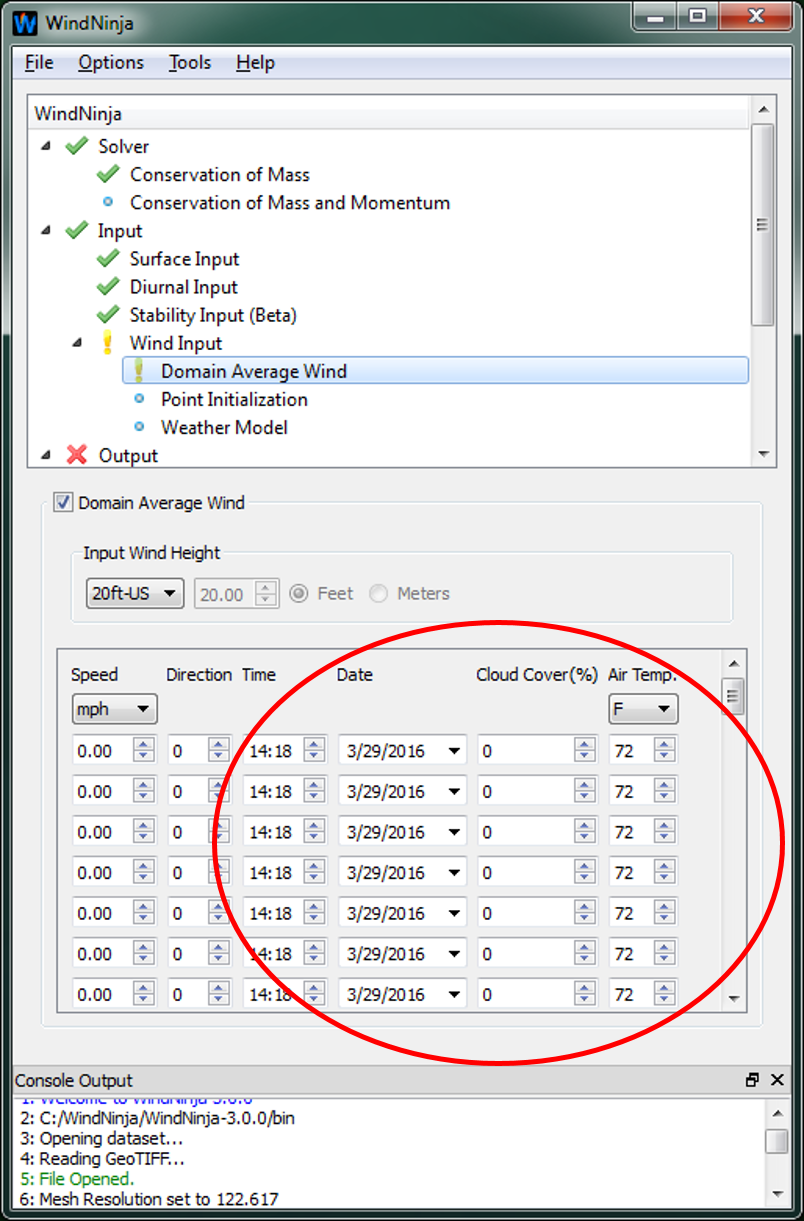
\includegraphics[scale=1.0]{imgs/domain_avg_1.png}
\end{figure}

These new input fields are “Time”, “Date”, “Cloud Cover”, and “Air Temp.”  The time should be specified in military time (24 hour format rather than 12 hour format).  A pop up calendar for entering the date can be accessed by left-clicking on the drop-down arrow on the right side of the date text box.  Cloud cover is the percent cloud cover (0-100\%).  A high percent cloud cover has the effect of reducing the diurnal wind speeds, day and night, by reducing radiant heat transfer between the sky and ground.  It will also tend to produce an atmosphere closer to neutral stability. The air temperature is the average air temperature over the simulation area.  Since the resulting diurnal winds are not very sensitive to the air temperature value, a value within $10^{\circ} - 15^{\circ}$ F of actual should be OK.

The domain average wind speed and direction will also need to be specified.  These are the same winds that were entered in \href{https://weather.firelab.org/windninja/tutorials/WindNinja_tutorial1.pdf}{WindNinja Tutorial 1: The Basics}.  During the wind computation, these winds will be combined with the diurnal winds to produce the final wind field.  Output of simulations done with light domain average winds (say 1-5 mph) will show significant effect of the diurnal winds.  Strong domain average wind cases will not show much diurnal effect because they are overpowered.  Note, however, that including diurnal winds in the simulation usually does not noticeably increase the solve time, so it is usually recommended for all simulations.  The general effect of the stability calculations will be more flow \textit{around} terrain features at night (stable atmosphere) and over terrain features during the day (unstable atmosphere).

\section{Output}

The same output files are written for diurnal and non-neutral stability simulations as non-diurnal simulations (Google Earth, Fire Behavior, Shape files, VTK files).  The only difference is in the output file naming convention.  Diurnal simulations also include the date and time in the filename.  You may want to review the different output file types in \href{https://weather.firelab.org/windninja/tutorials/WindNinja_tutorial1.pdf}{WindNinja Tutorial 1: The Basics} before continuing.

The image below is an example of the output file naming convention from a diurnal WindNinja run (color added for clarity).  The run used an ASCII Raster elevation file called “south\_canyon.asc”, an input direction of 270 degrees, input speed of 5 mph, date of 7/6/1994, time of 1200 local time, and an output file resolution of 200 meters.  The asterisk (*) at the end indicates that a file name extension would be here and would depend on exactly what type of output file this was (Google Earth would be “.kmz”, etc.).

\begin{figure}[H]
	\centering
	\label{}
	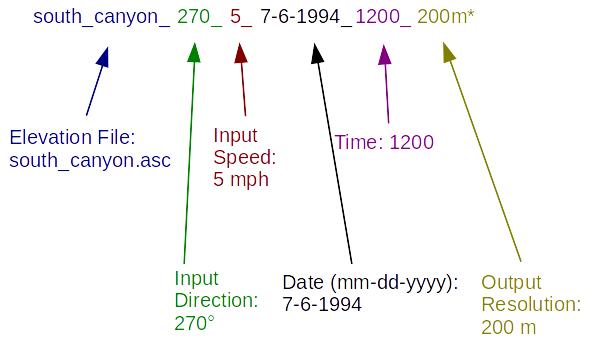
\includegraphics[scale=1.0]{imgs/colored_file_info_1.png}
\end{figure}

\textbf{\color{red}In the navigation tree, left-click on “Output” and select the “Output Height”, “Output Speed Units”, and  “Clip output by” values you want.}

\textbf{\color{red} Next, choose the types of output files you would like by left-clicking the type in the navigation tree and filling out the corresponding input panel.}

\section{Solve}

\textbf{\color{red} Left-click on “Solve” in the navigation tree.  Set the number of processors you would like using the “Number of Processors” text box.  Finally, left-click the “Solve” button to start the simulation(s).}

\textbf{\color{red} When finished, close the progress window.}

The simulations are complete!  The output files can be found in the folder where your elevation file is.  For your convenience, a button on the solve input panel called “Open Output Files Path” can be clicked to open your file browser in the folder where the output files were written.

\textbf{\color{red}  Left-click the “Open Output Files Path” button to see the output files that were written.}

This concludes \textbf{WindNinja Tutorial 2: Diurnal Winds}.



\end{document}